%
% File: chap03.tex
% Author: Oliver J. H. Feighan
% Description: Theory and parameterization for chl-xTB method. 
% Include vibronic PES tests, and absorption spectra.
%
\let\textcircled=\pgftextcircled
\chapter{Bespoke Chlorophyll Excited State Methods}
\label{chap:chl_xtb}

\subsubsection*{Previous Published Work}
All of the work presented in this chapter are also included in a paper published 
with Dr Susannah Bourne-Worster and Prof. Fred Manby in December 2022 \cite{Feighan2023}.

\initial {T}his chapter reports on designing and parameterising a novel method for
transition properties, referred to as Chl-xTB. The framework and theory for the method
is outlined in section \ref{sec:theory}. Parameterisation details are given in section \ref{sec:chl_params},
including the reference data used to create the training data, the objective function
and optimisation algorithms. The accuracy of this new method is showcased in the
final section \ref{sec:chl_benchmarking}.

From the previous chapter is was found that the tight-binding based \dxtb methods
are not the solution to LHC model issues outlined in the introduction. They are
too inaccurate, and the problem of comparing transitions to high-level methods makes
analysis difficult. Additionally, the issues with convergence to excited states 
with \dscf in general make these methods unreliable for many uses (e.g. for a correlated
set of structure where success with every time-frame is required.)

However, as found in the previous chapter, the sTDA-xTB method does imply that a 
tight-binding based approach would work, the only issue is the parameterisation of
the electronic structure method. In the introduction it was argued that sTDA-xTB
was not suitable for LHC exciton models as the minute variations in chlorophyll 
geometry may not be accurately treated - this claim is substantiated in section \ref{subsec:ref_data}.
This chapter posits that a method that is specific to chlorophyll would solve this
problem. The machine-learning models discussed in chapter \ref{chap:intro} are similar
in this respect, where models predicted only \Qy transition energies. Here it is
argued that electronic structure methods could fit this purpose instead of statistical
machinery, and would be much easier to parameterise and have more chemically significant
parameters, dependent on design choices in the excited state method. 

By keeping the excited state method "light-weight" (i.e. with few parameters and 
minimal computation), the efficiency of these methods may outstrip current approaches 
and match machine-learning methods. Additionally the risk of over-fitting to training 
data is reduced when using fewer parameters - compare the training set sizes of ML
methods, in the hundreds of thousands, to sTDA-xTB, which is in the hundreds. Fewer
parameters also increase the reusability of methods, as these parameters can be easily
re-optimised.

%=======
\section{Response and Electronic Structure Theory Approximations}
\label{sec:theory}

\subsection{Full TD-DFT Solutions}
\label{subsec:tddft_equation}
To recap full linear-response TD-DFT, excitation energies and transition characters 
are the given by the solutions of the non-Hermitian eigenvalue equation

\begin{equation}
    \begin{pmatrix}
        \mathbf{A}   & \mathbf{B} \\
        \mathbf{B}^\ast  & \mathbf{A}^\ast
    \end{pmatrix}
    \begin{pmatrix}
        \mathbf{X} \\
        \mathbf{Y}
    \end{pmatrix}
    = 
    \omega
    \begin{pmatrix}
        1 & 0 \\
        0 & -1
    \end{pmatrix}
    \begin{pmatrix}
        \mathbf{X} \\
        \mathbf{Y}
    \end{pmatrix}
\end{equation}
%
where $\mathbf{A}$, $\mathbf{B}$ are matrices whose elements describe the perturbation
of the electron density in response to light interaction, the $\mathbf{X}$, $\mathbf{Y}$
solutions are coefficients of excitations, similar to CIS, and eigenvalues $\omega$
are the excitation energies.

The elements of $\mathbf{A}$ and $\mathbf{B}$ correspond to descriptions of the
virtual-occupied and occupied-virtual contributions respectively, and in TD-DFT, 
with a global hybrid density functional, are given by

\begin{equation}
A_{ia,jb} = \delta_{ij} \delta_{ab} \left( \epsilon_a - \epsilon_i \right) + 2\left(ia|jb\right) - a_x\left(ij|ab\right) + (1- a_x)\left(ia|f_{\text{XC}}|jb\right)
\end{equation}
%
\begin{equation}
B_{ia,jb} = 2\left(ia|bj\right) - a_x\left(ib|aj\right) + (1- a_x)\left(ia|f_{\text{XC}}|bj\right)
\end{equation}
%
where indices $a,b$ and $i,j$ refer to virtual and occupied orbitals respectively,
$\epsilon_i$ is the orbital energy of orbital $i$, $a_x$ is the value of non-local
Fock exchange in the XC functional $f_{\text{XC}}$, and $\delta_{ij}$ is the Kronecker
delta function. The integrals (here in Mulliken notation) are Coulomb type for the
$\mathbf{A}$ matrix and exchange type for the $\mathbf{B}$ matrix. The leading term
in the $\mathbf{A}$ matrix is the orbital energy difference, which, due to the Kronecker 
delta functions, only contributes to the diagonal elements.

\subsection{Approximations to Full TD-DFT Solutions}
\label{subsec:chl_approxs}
\subsubsection{Tamm-Dancoff approximation and Diagonal Dominant $\mathbf{A}$ matrices}
\label{subsubsec:Tamm_Dancoff}

The first reduction to full linear response is the well-used Tamm-Dancoff approximation (TDA). 
TDA is one of the earliest approximations applied to full linear response theory, 
and outlines that only virtual-occupied contributions are considered when finding
roots of excitations \cite{Hirata1999}. The full casida equation in TDA theory is 
reduced to

\begin{equation}
\mathbf{A} \mathbf{X} = \omega \mathbf{X}
\end{equation}
%
where the definitions of elements are the same as above, but it should be noted 
that the solutions $\mathbf{X}$ will be different to full TD-DFT. This is formally
the same as a CIS problem, and has been reported as a way to get back to CIS from 
full TD-DFT \cite{Yoshimine1992, Hirata1999}.

As an eigenvalue problem, solving for $\omega$ requires constructing and diagonalizing
the full $\mathbf{A}$ matrix. Seen in equation \ref{eq:full_A_integrals}, the XC
functional is dependent on $\omega$ values and so iterating through diagonalisation
is needed to find stable, self-consistent solutions.

The success of \dscf demonstrates that solving the roots of the entire Casida equation
is sometimes unnecessary. In a similar spirit, a light-weight shortcut to solutions 
is the diagonal dominant approximation to eigenvalue solutions, where diagonal elements
of a matrix are taken as an approximation to the real solutions. By neglecting the
off-diagonal terms, this approach explicitly treats separate transitions as non-interacting,
as the off-diagonal elements describe the coupling between transitions in an excitation.
This approach is similar to the single-pole approximation (SPA) in this way \cite{Petersilka1996, Appel2006}.
Excitation energies would be then be given by

\begin{equation}
\omega_{ia} \approx A_{ia, ia} = \left( \epsilon_a - \epsilon_i \right) + 2\left(ia|ia\right) - a_x\left(ii|aa\right) + (1- a_x)\left(ia|f_{\text{XC}}|ia\right). 
\label{eq:diag_dom}
\end{equation}
%
If the integrals are assumed to be small compared to the first term, the orbital 
energy difference, then the orbital energy difference can be taken as an approximation 
to the full excitation energy, recovering the eigenvalue difference method explored 
in the previous chapter.

This approximation reduces computational cost by removing the need to calculate
all of the off-diagonal elements, as well as many diagonal elements for transitions
that are not of interest. This approach would be expected to work best where the
overall transitions are not mixed. If transitions are mixed, then the coupling elements
would be non-zero, and depending on the proximity in energy of single transitions,
the coupling values could have a large effect. This is considered in section \ref{subsec:qy_transition}.

\subsection{Integral Approximations with Monopole Expansions}
\label{subsec:MNOK}

Whilst using a diagonal dominant approximation removes a large portion of the integrals,
those that are left would still require an iterative, self-consistent treatment. 
This can be simplified by approximating these integrals as point charge interactions, 
as charges would not be dependent on excited state solutions.

Atom centered transition charges for transition $m \rightarrow n$ can be given in
the Mulliken scheme by summing the reduced one-electron transition density $\mathbf{D}^{mn}$
multiplied by the orbital overlap $\mathbf{S}$ for all orbitals $p$, $q$ centred
on atom $A$

\begin{equation}
q^{mn}_A = \sum_{p \in A} D^{mn}_{pq} S_{pq}  
\end{equation}
%
Partial charges can be given as the difference between the electronic charge
and the nuclear charge $Z_A$

\begin{equation}
q_A = Z_A - \sum_{p \in A} D_{pq} S_{pq}  
\end{equation}
%
where $\mathbf{D}$ is the reduced one-electron density. This applies to any state,
so can be used to calculate ground state and excited state partial charges.

MNOK operators can recover the important behavior of full electron integrals that
is lost in classical charge-charge interaction, especially for the small distance limit \cite{Grimme2016}.
For both Coulomb and exchange type integrals, this can be done with a short-range
damped MNOK operators. The integral is approximated by

\begin{equation}
\left(pq|rs\right) \approx \frac{1}{2}\sum^N_A \sum^N_B q_A^{mm} q_B^{mn} \Gamma_{AB}
\end{equation}
%
where $N$ is the total number of atoms in the system and $p$,$q$,$r$, $s$ are electron
indices for both occupied and virtual orbitals, and $A$ and $B$ are indices for
 the atoms. For Coulomb type integrals, the operator $\Gamma_{AB}$ is given by

\begin{equation}
\Gamma^J_{AB} = \left(\frac{1}{\left(R_{AB}\right)^{y_J} + \left(a_x \eta\right)^{-y_J}} \right)^{\frac{1}{y_J}}
\label{eq:gammaJ}
\end{equation}
%
where $R_{AB}$ is the interatomic distance and $\eta$ is the average of the chemical 
hardnesses. The chemical hardness of a given atom is defined as

\begin{equation}
\eta\left(A\right) = \frac{\delta^2 E\left(A\right)}{\delta^2 N^2}
\end{equation}
%
but in practice is precomputed and used as a static parameter. $y_J$ and $a_x$ are
global parameters, with the latter used to recover the effects of Fock-exchange
mixing in the short-distance limit. For exchange type, the operator is

\begin{equation}
\Gamma^K_{AB} = \left(\frac{1}{\left(R_{AB}\right)^{y_K} + \eta^{-y_K}} \right)^{\frac{1}{y_K}}
\label{eq:gammaK}
\end{equation}
%
where the $y_K$ parameter replaces the $y_J$ parameter in the Coulomb type operator.

As the $a_x$ parameter can account for many of the exchange effects, the density 
functional in equation \ref{eq:diag_dom} is also neglected to further reduce computational 
cost. The final form of the expression used to calculated excitation energies is 
then given by

\begin{equation}
\omega_{ia} = \left(\epsilon_a - \epsilon_i\right) + \sum^N_{A,B}\left(2 q_{ia}^A \Gamma^K_{AB} q_{ia}^B - q^A \Gamma^J_{AB} q^B\right)
\end{equation}
%
where the exchange term uses transition charges $q_{ia}$, and the Coulomb term uses
partial charges from the ground state density.

It can be seen that the inclusion of MNOK operators introduces global parameters
These would require optimisation to a training set. Initially it was investigated
whether parameterising to a training set with a broad range of systems and transitions
would be possible. However it was found that parameter optimisation procedures, 
whilst improving upon the accuracy of the \dxtb methods of the previous chapter,
could not break into the accuracy needed to investigate chlorophyll systems well
enough (discussed in more detail in \ref{subsec:ref_data}). This is due to many
transitions being mixed, which would not be consistent with conditions needed for
the diagonal dominant approximation. Additionally, issues with autonomous optimisation
assigning transitions without symmetry made optimisation workflows difficult (see
section \ref{subsubsec:post_scf_symmetry}).

However a method that works for a wide set of systems is not required for LH2,
as only the \Qy transition is of interest for many models. Parameterising to a 
single, well-defined transition would be a much better approach for this investigation.
By reducing the scope of systems, the specificity of parameters can dramatically increase. 
This reduces the need to include more parameters to improve accuracy, as well as 
decreasing the amount of training data needed. Looking at other transitions and
systems then is outside the scope of this work, but could be a large area for further
work for similar investigations. An outline of the \Qy transition, and its applicability
to these approximations, is given below.

\subsection{The \Qy Transition}
\label{subsec:qy_transition}
\begin{figure}
    \centering
    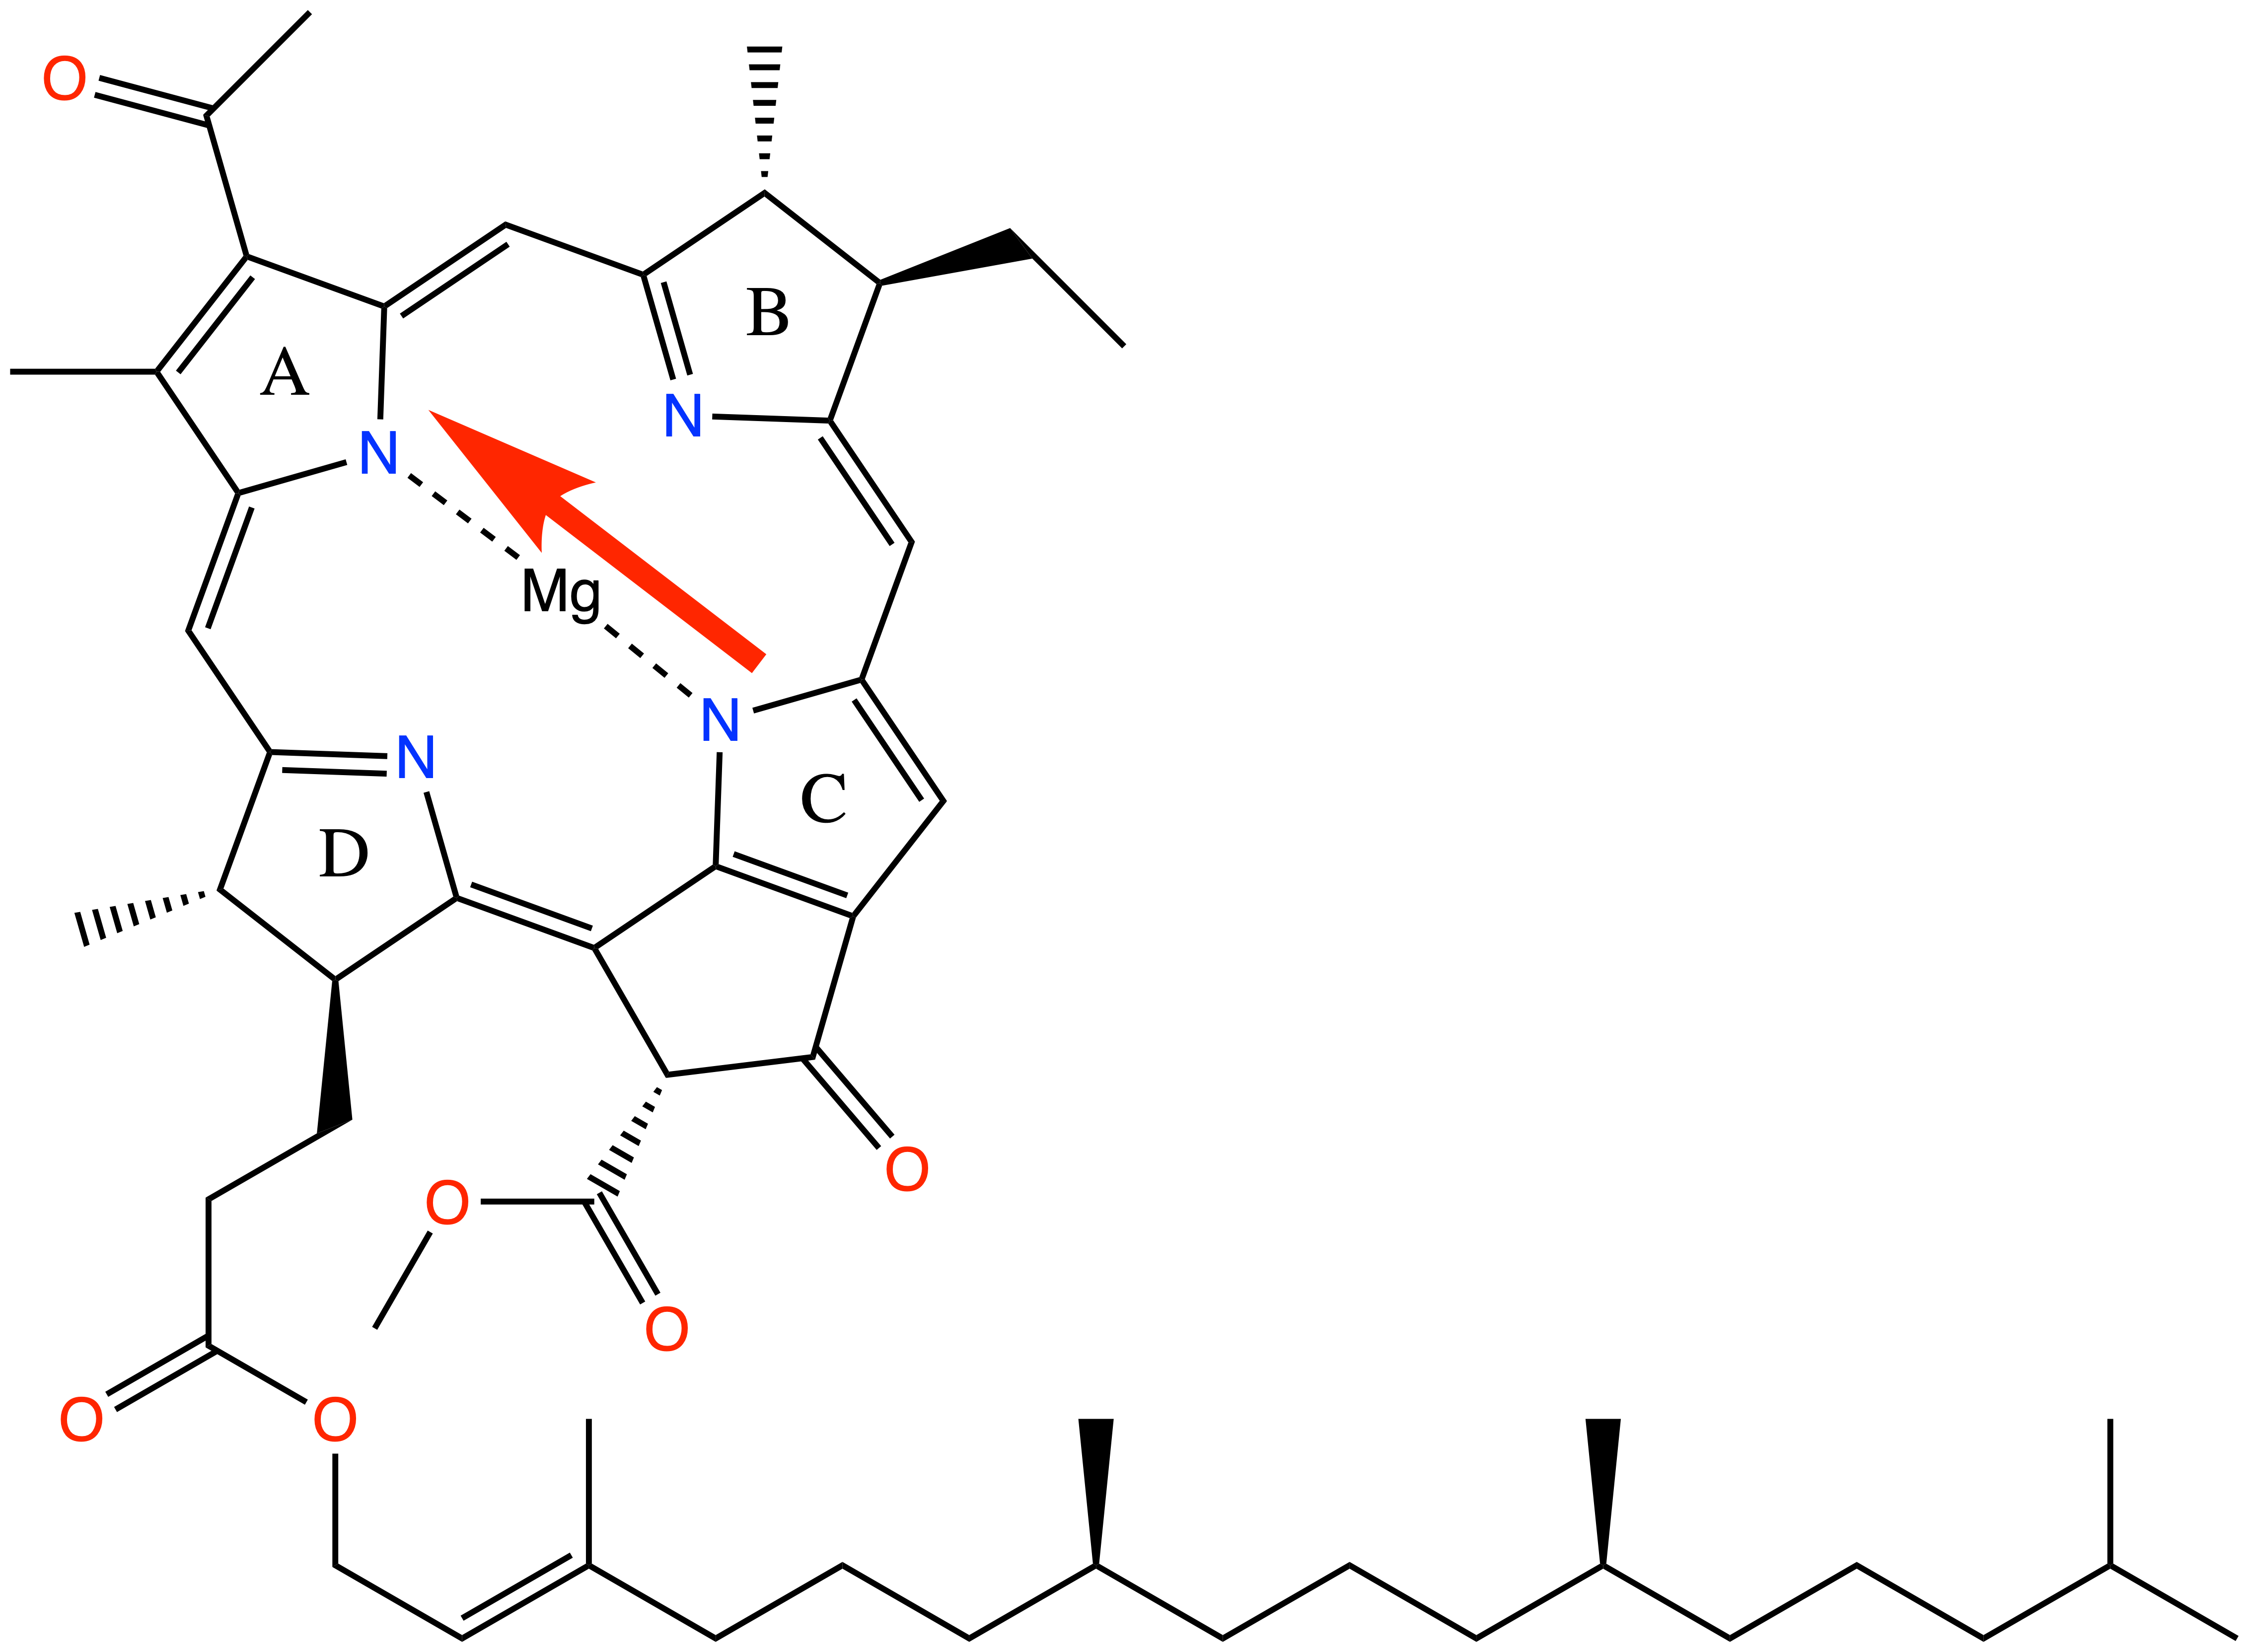
\includegraphics{chapters/4_chl_xtb/chlorophyll_Qy.png}
    \caption{Bacterial Chlorophyll a (BChla) with a model \Qy transition dipole.}
    \label{fig:bchla_qy}
\end{figure}

The \Qy transition is a good candidate to test approximations to full linear response 
theory. It is a well-defined transition which makes assignment easy, and has been
thoroughly analyzed in the literature \cite{Strain1963, BelenOviedo2011, Zucchelli2002, Kim2020, Sirohiwal2020}. 
It is also one of the most important transitions in light harvesting systems so 
an accurate treatment is necessary for high-performing LHC models.

The \Qy transition is one of the two transitions that make up the $Q$ band in the
absorption spectra of chlorophyll, the other being the $Q_x$ transition \cite{Sirohiwal2020}.
It is well known that the \Qy transition is important for electronic energy transfer, 
and predicting both transition energies and dipole moments correctly is important 
in constructing  frameworks that model this transfer \cite{Zazubovich2001}. The
\Qy transition is mostly HOMO-LUMO in character (~96\%), with a small amount of 
HOMO-1 - LUMO+1 (remaining 4\%) \cite{Saito2020}. The analogous transition in the 
unsubstituted tetraphorphyrin ring has the transition dipole along the molecular
axis defined by the N atoms \cite{Fragata1988}, however due to the asymmetry introduced
by substitutions and geometry deformations, BChla \Qy transitions have a deviation
to this axis of around 12 $^{\circ}$ \cite{BelenOviedo2011}. In this was the \Qy
transition in chlorophyll lies mostly mostly along the $N_A$-$N_C$ axis, with $Q_x$
lying orthogonally along the $N_B$-$N_D$ axis. $Q_x$ has the reverse character to
the \Qy transition, being mostly HOMO-1 - LUMO+1.

Plots of the electron density of the HOMO and LUMO show how this transition is delocalized
over large sections of the porphyrin ring, with approximate $C_2$ symmetry along
the molecular axes. Notable contributions can be seen in the functional groups,
giving the modified transition behavior seen in different versions of chlorophyll \cite{BelenOviedo2011}.

\begin{figure}
    \centering
    \includegraphics[scale=0.4]{../../Year_2/chlorophyll_parameterization/cube_files/HOMO_copy.png}
    \caption{The HOMO orbital of Bchla from PBE0/Def2-SVP DFT.}
    \label{fig:HOMO}
\end{figure}

\begin{figure}
    \centering
    \includegraphics[scale=0.4]{../../Year_2/chlorophyll_parameterization/cube_files/LUMO_copy.png}
    \caption{The LUMO orbital of BChla from PBE0/Def2-SVP DFT.}
\end{figure}

It has recently also been shown that the high correlation between the eigenvalue
difference of HOMO-LUMO orbitals and full TD-DFT excitation energies implies that
the HOMO-1 - LUMO+1 transition can be excluded from the transition character \cite{Saito2020}.
This is also supported by the results for the chlorophyll test set in the previous
chapter as \dscf with its single transition treatment is able to capture \Qy transitions
with good accuracy.

The high amount of single-transition character in the \Qy transition makes it ideal
for the approximations to transition energies set out so far. The lack of coupling
elements that would appear in the $\mathbf{A}$ matrix justifies the use of the diagonal
dominant approximation.

Additionally, the well-defined transition makes assignment trivial, and the transition
dipole orientation to the $N_A$-$N_C$ axis has been used as a metric for the accuracy
of transition dipole moments. As a singular value this is ideal for autonomous optimisation,
both for use in an objective function as well as for discarding outlier transitions.

\subsection{Bespoke xTB Parameters for Chlorophyll}
\label{subsec:chl_method}

As found in the last chapter, the underlying electronic structure can have a huge
effect on the accuracy of transition properties. The GFN-xTB methods in particular,
both linear response and \dxtb, were ill-suited for transition properties. Whilst
DFT methods could have been used as for Mulliken partial and transition charges,
this would not be any more efficient that the \dscf methods discussed in the previous 
chapter. A tight-binding, semi-empirical approach for the electron structure is still 
required. To improve the applicability of the xTB methods for transition properties, 
some of the parameters would need to be altered. A top-down approach can be used 
for these alterations, as it has been shown to work well for the GFN-xTB and sTDA-xTB
methods. 

As discussed in the introduction chapter, the GFN1-xTB Fock matrix is made of both
charge-dependent and charge-independent terms. The form of these terms, and definitions
of parameters, are also given in chapter \ref{chap:background_theory}. Only the
charge dependent terms would have any effect on the partial and transition charges,
thereby affecting the transition properties. The charge dependent terms are the 
first, second and third density fluctuation terms. The first order term is the leading 
term, and so altering parameters in this term would have the greatest effect. Only
some of these parameters are "free", with others calculated from physical or \emph{ab initio}
values. The "free" parameters are the H{\"u}ckel parameters $k_l$, where $l$ is
the angular momentum of the orbital, and the global scaling parameters. The global
scaling parameters are used to adjust interactions for some pairs of elements where
the global parameters led to erroneous properties, usually observed in the bond
lengths. It was found that for the \Qy transition, only Mg and N interactions had
to be scaled.

An obvious drawback of altering these parameters to fit transition properties is
that they would lose their specificity to the GFN-xTB training set. However it is
not required, or in the scope of this work, to find a semi-empirical method that 
would be able to calculate all properties for chlorophyll. The planned uses for
approach do not include calculating optimised geometries or hessians of chlorophyll
in this work, as other methods would be expected to much perform better. Including
more target properties into the parameter optimisation would decrease the accuracy
to any one target, arguably making the method worse overall. For example, the sTDA-xTB 
and GFN-xTB methods use different electronic structure parameters for this reason - 
one for transition properties, the other for geometries.

The combination of specification to chlorophyll transition properties and using 
xTB electronic structure lends this specific method to be named Chl-xTB. However
this is only a realization of an excited state method using the protocol outlined
here. Discussion of application to other systems can be found in chapter \ref{chap:discussion}.

\subsection{Transition and Excited State Density from the Ground State}
\label{subsec:trans_excited_densities}

Similar to \dscf, the ground state orbital coefficients are taken to be a good approximation
to the (\Qy) excited state coefficients. It was assumed that the excited state could
be calculated without orbital relaxation, so that both the excited state and ground
state could be constructed from the same set of molecular orbitals. The transition
density is then calculated as

\begin{equation}
\mathbf{D}^{01} = \ket{\Psi^0} \bra{\Psi^1} 
\end{equation}
%
with $\bra{\Psi^0}$, $\bra{\Psi^1}$ (the ground and excited state respectively)
being constructed from the same set of molecular orbital coefficients $\mathbf{C}$
but with different sets of occupation numbers for the ground and excited state (
labelled $n^{\left(0\right)}$ and $n^{\left(1\right)}$ respectively). The ground state
and excited state density can be similarly calculated as

\begin{equation}
\mathbf{D}^{\left(0\right)} = \sum_i n^{\left(0\right)}_i C^{\left(0\right)}_{ip} C^{\left(0\right)}_{iq}
\end{equation}
%
\begin{equation}
    \mathbf{D}^{\left(1\right)} = \sum_i n^{\left(1\right)}_i C^{\left(0\right)}_{ip} C^{\left(0\right)}_{iq} 
\end{equation}
%
These density matrices are used to calculate the partial and transition charges
with the Mulliken scheme, which is in turn used to calculate the MNOK integrals.
The transition and molecular dipoles can be calculated as the trace of the dipole
operator with the density.

It should be noted the ground and excited states would be orthogonal in this scheme,
as they share the same set of MO coefficients. Additionally, the problematic excited
state convergence is unnecessary as only the ground state cycle of the SCC procedure 
is needed. Excited state properties, such as the molecular dipole and partial charges 
can also be calculated from the excited state density, which will be important for 
the exciton framework of the next chapter.

It was found, however, that transition dipoles calculated using this method were
much larger than TD-DFT. This was also observed for the \dscf and eigenvalue
difference methods, implying that the inclusion of the HOMO-1-LUMO+1 transition
is key to accurately describing the transition density and its magnitude. To recover
correct magnitudes, an additional parameter $D_scl$ was included to scale the transition
density (i.e. $\tilde{D}^{Q_y} = D_{\text{scl}} D^{01}$  where $\tilde{D}$ is the
scaled transition density ) which both yielded the correct transition dipole magnitudes
as well as drastically increasing the accuracy of the method overall.

\afterpartskip
\section{Parameterization}
\label{sec:chl_params}
An objective function and algorithm are required to find minima in parameter space,
where these minima correspond to an optimized set of parameters. Reference data 
are also required as a target. All of these elements are important for minimizing 
the amount of error in the final method, as well as determining how well a method 
can perform when used for different problems.

\subsection{Objective Function}
\label{subsec:obj_func}
The first metric chosen to be minimised was the root mean squared error (RMSE), 
where the error is against reference transition energies, giving the objective function 
as

\begin{equation}
f_{\text{RMSE}}\left(\mathbf{x}\right) = \sqrt{ \frac{1}{N} \sum^N_i \left( \Delta E_i  - \Delta E_{i, \text{ref.}}\right)^2}
\end{equation}
%
where $\textbf{x}$ is the set of parameters, $\delta E_i$, $\delta E_{i,\text{ref.}}$ 
are the transition energies for system $i$ from the chl-xTB method and reference
method respectively, $N$ is the number of systems used to calculated the objective
function value (this can be different when looking at training and testing sets).

However just using the RMSE has two issues. First is that other transition properties
are not included in the optimisation, and so no comments can be made on the accuracy 
of, for example, transition dipoles. This can be fixed by including a metric for
the error in other properties of interest. The other issue is that a low RMSE does
not guarantee a high correlation. A measure of the correlation can be given by the
coefficient of determination

\begin{equation}
R^2 = 1 - \frac{\sum^N_i \left(\hat{y}_i - y_i \right)^2}{\sum^N_i \left(\hat{y}_i - \bar{y}\right)^2}
\end{equation}
%
where $\hat{y}$, $y$ are the predicted and reference values respectively and $\bar{y}$
is the average of the reference values. The correlation is a better metric for determining
if chl-xTB has a small enough random error to predict transition properties, however
it may not account for systematic errors. Both a low RMSE and high $R^2$ value are
needed to optimise fully to the reference data, and the two metrics are not fully
mutually inclusive.

By including both RMSE and $R^2$ values, for transition energies as well as dipole
magnitudes, the full objective function becomes

\begin{equation}
f_{\text{full}} \left( \mathbf{x} \right) = \lambda_1 \text{RMSE} \left(\Delta E \right)+ \lambda_2 \text{RMSE}\left( \left| \mu \right| \right) + \lambda_3 \left(1 - R^2 \left( \Delta E \right)\right) + \lambda_4 \left( 1 - R^2 \left( \left| \mu \right| \right)\right)
    \label{eq:obj_func}
\end{equation}
%
where $\lambda_n$ are weights necessary to keep all of the terms to a similar range.
This provides stability to the optimisation procedure, such that no one term dominates
the solution space.

\subsection{Minimisation Algorithms}
\label{subsec:algorithms}
Finding the optimal parameters for the Chl-xTB method is a nonlinear problem. The
parameters so far discussed can not be used to create a linear function that would
reproduce the value of the objective function. Therefore it is necessary to use 
heuristics that can solve non-linear problems.

\subsubsection{Nelder-Mead}
\label{nelder_mead}
The Nelder-Mead method, as implemented in \code{SciPy}, is a modified version of a simplex
algorithm, that uses a $n$-dimensional shape to define a test region, and iteratively
searches the $n$-dimension space by reflecting the vertices of the test region. 
The test region, or more specifically the shape described by its vertices, is the
simplex. The simplex has $n+1$ vertices - for example, a 2-dimensional problem
would have a triangular simplex.
The algorithm starts with an initial simplex guess. It is important that the initial
guess covers enough area to avoid descending into any local minima, whilst not being
too large as to not take into account finer details of the parameter space. Minima
in the complex space are found by propagating the simplex, either by expanding,
contracting, shrinking or reflecting around a a central value defined by the set
of vertices. For example to find the parameters $\mathbf{x}$ that correspond to 
a minimum of the function $f\left(\mathbf{x}\right)$

\begin{equation}
\min_{\mathbf{x} \in \mathbb{R}^n} f\left( \mathbf{x} \right)
\end{equation}
%
with initial simplex vertices $\mathbf{x}_1, \dots, \mathbf{x}_{n+1}$, the first 
step is to order the function values of the vertices

\begin{equation}
f\left(\mathbf{x}_1\right) \leq f\left(\mathbf{x}_2\right) \leq \dots \leq f\left(\mathbf{x}_{n+1}\right)
\end{equation}
%
and calculate the centroid of the set of vertices, excluding the worst vertex 
$\mathbf{x}_{n+1}$. The next steps then propagate the simplex, first by testing 
whether a reflection point $\mathbf{x}_r$ is better than the worst vertex used to
calculate the centroid

\begin{equation}
\mathbf{x}_r = \mathbf{x}_0 + \alpha\left(\mathbf{x}_0 - \mathbf{x}_{n+1}\right) 
\end{equation}
%
where $\mathbf{x}_0$ is the centroid point. There are then a set of three possibilities
for the value of $f\left(\mathbf{x}_r\right)$. First is that it is the best value
found so far, and so the simplex should be expanded along the centroid-reflected 
vertex axis

\begin{equation}
\mathbf{x}_e = \mathbf{x}_0 + \gamma\left(\mathbf{x}_r - \mathbf{x}_0 \right).
\end{equation}
%
The corresponding vertex of the two function values $f\left(\mathbf{x}_r\right)$, 
$f\left(\mathbf{x}_e\right)$ then replaces the "worst" vertex $\mathbf{x}_{n+1}$.

A second possibility is that the function value for the reflected vertex is better
than the worst vertex used to calculate the centroid, but worse than the best 
value, $f\left(\mathbf{x}_1\right) \leq f\left(\mathbf{x}_r\right) \leq f\left(\mathbf{x}_n\right)$.
In this case the $\mathbf{x}_{n+1}$ vertex is replaced by the reflected vertex.

The last possibility is that the reflected vertex has a greater function value than
any vertex used to calculate the centroid. In this case a new point (contraction),
or set of points (shrink) are used to propagate the simplex. Depending on whether
this function value is greater or less than the worst vertex in the simplex ($\mathbf{x}_{n+1}$),
the contracted point is either inside or outside of the simplex

\begin{equation}
    f\left(\mathbf{x}\right)= 
    \begin{cases}
    \mathbf{x}_c = \mathbf{x}_0 + \rho \left(\mathbf{x}_r - \mathbf{x}_0 \right)               & \text{if } f\left(\mathbf{x}_r\right) < f\left(\mathbf{x}_{n+1}\right)\\
    \mathbf{x}_c = \mathbf{x}_0 + \rho \left(\mathbf{x}_{n+1} - \mathbf{x}_0 \right)           & \text{otherwise } f\left(\mathbf{x}_r\right) \geq f\left(\mathbf{x}_{n+1}\right)
    \end{cases}
\end{equation}
%
if the contracted point $\mathbf{x}_c$ is give a smaller function value than the 
reflected point for the first case, or the worst point for the second case, it then
replaces the worst simplex vertex.

The final possibility is that both the contracted point function value is greater 
than either the reflected point or the worst point. In this case, the entire simplex
is shrunk around axes to the best vertex

\begin{equation}
\mathbf{x}_i = \mathbf{x}_1 + \sigma \left(\mathbf{x}_i - \mathbf{x}_1 \right)
\end{equation}
%
for $i \in \{1, \dots, n\}$.

Once either the worst vertex or all of the vertices are replaced, the new simplex
is used as the start of a further iteration. Iterations are stopped once a termination
criterion is met, such as a vertex function value being below a threshold.

Several versions of this method exist, that add additional constraints. This can
include keeping the volume of the simplex constant, which can promote a steepest
descent approach.

\subsubsection{Sequential Least-Squares Quadratic Programming}
\label{subsubsec:slsqp}
The sequential least-squares quadratic programming (SLSQP) method is fundamentally
different to the previous Nelder-Mead method, and follows a quasi-Newton procedure
with additional factors to treat constraints.

The general problem is similar to Nelder-Mead, namely to solve

\begin{equation}
\min_{\mathbf{x} \in \mathbb{R}^n} f\left( \mathbf{x}\right)
\end{equation}
%
however with an arbitrary amount of constraint functions $c$

\begin{equation}
c_i \left(\mathbf{x} \right) = 0
\end{equation}
\begin{equation}
c_j \left(\mathbf{x} \right) \leq 0
\end{equation}
%
where $i$, $j$ are indices of the constraint functions.
It is assumed that the space of $f$ and $c_n$ are one-to-one mappable on the
space of $x$, and also is continuously differentiable. Starting from an initial
value of $\mathbf{x}_0$, a search direction $d^k$ and step length $\alpha_k$ are
used to propagate the set of parameters by

\begin{equation}
\mathbf{x}_{k+1} = \mathbf{x}_k + \alpha_k \mathbf{d}_k
\end{equation}
%
The search direction, analogous to the ratio of function value to gradient in the
Newton-Raphson method, is calculated by solving the Lagrange function

\begin{equation}
\mathcal{L} \left(\mathbf{x}, \lambda\right) = f\left(\mathbf{x}\right) - \sum^m_n \lambda_n g_n \left( \mathbf{x}\right)
\end{equation}
%
with a quadratic approximation, that reduces the problem to a quadratic programming
subproblem

\begin{equation}
\min_d f\left(\mathbf{x}_k\right) + \nabla f\left(\mathbf{x}_k\right)^T d + \frac{1}{2}d^T \nabla^2_{xx} \mathcal{L} \left(\mathbf{x}_k, \lambda_k \right) d
\end{equation}
%
where the last term is often short-handed as the $\mathbf{B}$ matrix. This is the 
sequential quadratic programming method. A linear least squares subproblem could
be used instead of quadratic programming, which in would give the subproblem as

\begin{equation}
\min_d \left\| \left(\mathbf{D}_k\right)^{\frac{1}{2}} \left(\mathbf{L}_k\right)^T d + \left(\mathbf{D}_k\right)^{-\frac{1}{2}}\left(\mathbf{L}_k\right)^{-1}\nabla f \left(\mathbf{x}_k\right)\right\|
\end{equation}
%
where the matrices $\mathbf{L}$, $\mathbf{D}$ are from a diagonal decomposition 
of $\mathbf{B}$

\begin{equation}
\mathbf{L}_k \mathbf{D}_k \left(\mathbf{L}_k\right)^T = \mathbf{B}_k
\end{equation}
%
With the solutions for $\mathbf{d}_k$ solved by these subproblems, the parameter 
vector $\mathbf{x}$ can be propagated until similar termination criteria as the 
Nelder-Mead method.

A visualization finding a parameter set $\mathbf{x}$ corresponding to a local minimum
of the Himmel-Blau function \cite{Himmelblau1972} (a standard benchmark for optimisation 
algorithms) is shown in figures \ref{fig:nelder_mead} and \ref{fig:slsqp}. The former 
shows the Nelder-Mead simplex vertices, with the latter showing iterations in the 
$\mathbf{x}$ space. It can be seen that the Nelder-Mead algorithm evaluates more
points and covers a broader space, whereas the SLSQP algorithm follows a more direct
gradient descent. 

Both these methods were used to find optimal chl-xTB parameters, and it was found 
that the SLSQP method performed best, both in terms of the number of iterations,
stability, and in the overall value of the objective function. This could be due 
to the addition of constraints, however it is hard to say as the wrapping of \code{SciPy}
make both methods black-boxes that are hard to investigate further. The results
of the optimisation is discussed in further detail in section \ref{subsec:chl_opt_results}.

\begin{figure}
    \centering
    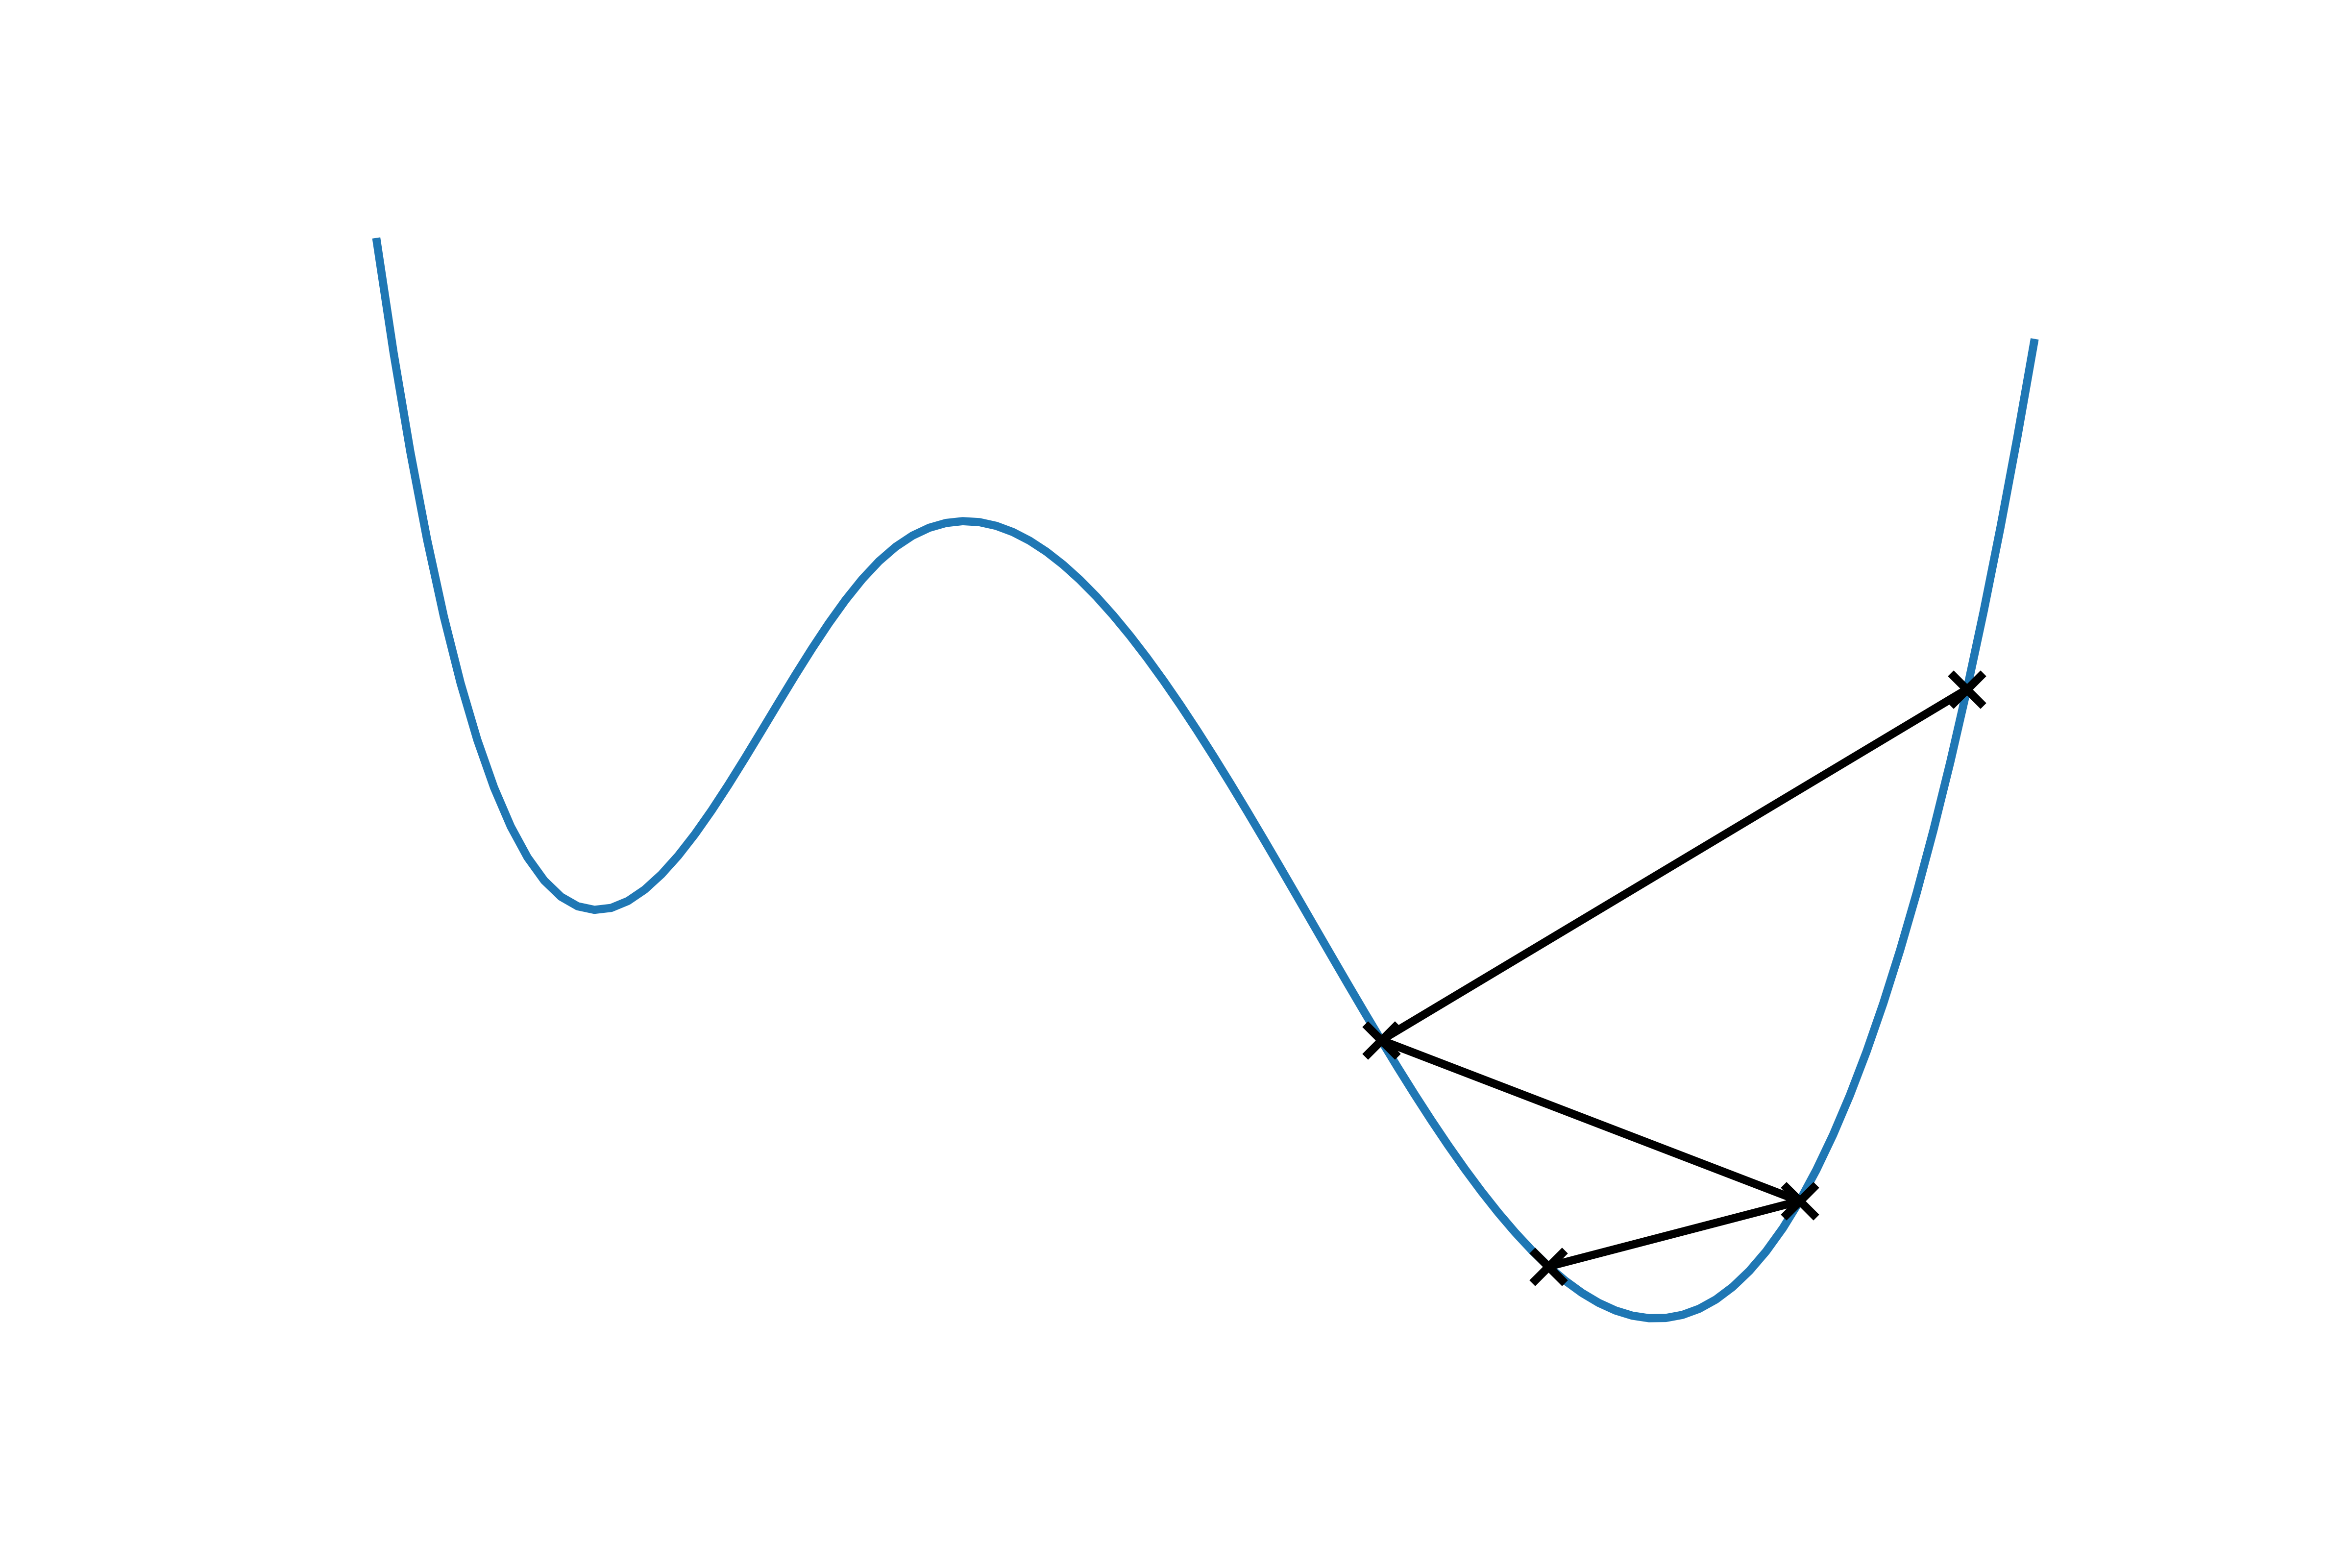
\includegraphics[scale=0.4]{nelder-mead.png}
    \caption{An example of the search through solution space using the Nelder-Mead
    method. The scatter points are positions of the Nelder-Mead simplex vertices,
    attempting to find the coordinates of the minimum in the Himmelblau function.}
    \label{fig:nelder_mead}
\end{figure}

\begin{figure}
    \centering
    \includegraphics[scale=0.4]{SLSQP.png}
    \caption{A similar example of the search through solution space, but using the
    SQSLP method. The scatter points are positions of the iterative solution vector
    $\mathbf{x}$, again attempting to find the coordinates of the minimum in the 
    Himmelblau function.}
    \label{fig:slsqp}
\end{figure}

\subsection{Reference Data}
\label{subsec:ref_data}
The geometries for the training set used to optimize the chl-xTB method were taken
from molecular dynamics of the LH2 protein used by Manby \emph{et al.} \cite{Stross2016}. 
The geometries of LH2 were chosen from uncorrelated snapshots, although each of
the 27 chlorophylls from each snapshot were included in the training data to give 
appropriate weighting to the differences in binding pockets. The stochastic collection 
of LH2 snapshots was chosen to cover a range of chlorophyll conformations to reduce
the amount of artificial bias towards any particular correlation of geometries.

Training the chl-xTB parameters was done against PBE0 data. These data were chosen
for the best accuracy-cost ratio, as well as having been previously used to investigate
exciton properties for the LH2 system \cite{Stross2016}. Additionally, from the
outset it was unknown how much training data would be necessary, and so keeping 
potential future costs of expanding the training data down was another factor in 
choosing this functional.

\afterpartskip
\begin{table}
    \centering
    \begin{tabular}{|| c | c | c | c | c ||}
    \hline
                        & $\text{RMSE}\left(\Delta E\right)$ / eV & $R^2\left(\Delta E\right)$ & $\text{RMSE}\left(\lvert \mu \rvert\right)$ / $e a_0$ & $R^2\left(\lvert \mu \rvert\right)$ \\
    \hline
    PBE0                & 0.147 & 0.795 & 0.172 & 0.919 \\ 
    $\omega$-B97XD      & 0.053 & 0.972 & 0.043 & 0.993 \\
    BLYP                & 0.098 & 0.554 & 0.543 & 0.080 \\
    \dscf               & 0.079 & 0.764 & 1.283 & 0.646 \\
    $\Delta \epsilon$   & 0.363 & 0.790 & 1.341 & 0.610 \\
    ZINDO               & 0.449 & 0.735 & 1.354 & 0.623 \\
    sTDA-xTB            & 0.517 & 0.258 & 0.843 & 0.151 \\
    \hline
    \end{tabular}
    \caption{Summary of the errors and correlations of transition properties for 
    \Qy for a set of LH2 BChla geometries from a range of established respond methods.
    The errors were calculated against CAM-B3LYP/Def2-SVP TD-DFT data, for transition
    energies ($\Delta E$) and transition dipole moments ($\left\lvert\mathbf{\mu} \right\rvert$).}
    \label{table:ref_data}
\end{table}

Transition properties were calculated with a range of methods, covering different
levels of theory and response methods. These include an eigenvalue difference approach,
\dscf, and TD-DFT with different levels of theory. This comparison was done so that
the performance of any parameterisation results could be benchmarked with an idea
about accuracy expectations.

The errors and correlations of the reference data are shown in table \ref{table:ref_data}.
The methods included in the benchmarking were \dscf, TD-DFT and eigenvalue difference
all using the PBE0 functional and Def2-SVP basis set. Also included are $\omega$-B97XD
and BLYP functionals with Def2-SVP basis sets, as a higher and lower level TD-DFT
reference respectively. The basis set was not changed as it has been found that 
the basis set has less importance on the accuracy than the functional \cite{Stross2016}. 
Also included are ZINDO and sTDA-xTB to represent other efficient response methods.

There are large variations in correlation and RMSE values for the reference methods
compared to CAM-B3LYP. This variation sets a reasonable expectation of how well
a new method might perform. The $\omega$-B97XD functional performs best with an 
RMSE of 0.053 eV, and is the most correlated (of the TD-DFT methods) with an $R^2$
value of 0.972. The other TD-DFT methods have similar accuracies ranging from 0.079
eV to 0.147 eV. Good accuracy is not followed by high correlation (see PBE0 with 
the highest RMSE but highest $R^2$ past $\omega$-B97XD), which illustrates how a
low RMSE and high correlation are not mutually inclusive and so must both be present
in the objective function. 

The variance in these different TD-DFT methods, all of which have been used in studies
on chlorophyll, show how it is difficult to assign a true value to transition energy
for a set of geometries. Therefore as long as the accuracy of chl-xTB is within 
the range of methods shown here, it would also be valid.

The single transition methods also perform well, corroborating the earlier statement
that only treating a HOMO-LUMO transition can give accurate results. \dscf performs
as well as any of the TD-DFT methods with an RMSE and $R^2$ values of 0.079 eV and
0.764 respectively. Whilst the eigenvalue difference method has a higher RMSE at
0.363 eV its correlation of 0.79 is still similar to the TD-DFT methods. Hence,
due to the dominance of HOMO-LUMO transition character, treating the transition
as mixed is not necessary in order to achieve accuracy for transition energies. 
The story for transition dipoles, however, is different.

The agreement of transition dipole magnitudes is much lower than excitation energies.
The RMSE of \dscf and eigenvalue difference methods is significantly higher (1.283
a.u. and 1.241 a.u. respectively) than the TD-DFT methods (0.172 a.u., 0.043 a.u.
and 0.543 a.u. for PBE0, $\omega$-B97XD and BLYP respectively). The average magnitude
of PBE0 transition dipoles is 2.751 a.u., with the average for \dscf and eigenvalue 
difference being 4.287 a.u. and 4.342 a.u. respectively. This disparity is attributed
to the lack of inclusion of $Q_x$ transition character. As the direction of the dipole
of this transition is orthogonal to \Qy it may reduce the transition dipole magnitude, 
similar to the effect seen in the outliers in the previous chapter.

Whilst there is a high degree of correlation between the higher level TD-DFT methods
(0.919 and 0.993 for PBE0 and $\omega$-B97XD respectively) the other methods
have a much lower correlation to PBE0 transition dipoles. BLYP is the worst correlated,
with a $R^2$ value of 0.080, which is fully uncorrelated. \dscf and eigenvalue difference
show a slight correlation at around 0.6-0.65.

Also included in the benchmarking was the semi-empirical method ZINDO. This had a
poor accuracy but reasonable correlation, with RMSE and $R^2$ values of 0.449 eV 
and 0.735 for transition energies, and 1.354 a.u. and 0.623 for transition dipoles.
sTDA-xTB also performs poorly, with the highest RMSE at 0.517 eV and with a low 
correlation of 0.258. This supports the arguments made in \ref{subsec:stda_xtb}
and demonstrates how this method is not suitable this study. These two methods act
as a benchmark for how well a more efficient response method could be expected to
perform.

Overall an RMSE to transition energies and dipoles of ~0.15 eV and ~0.2 a.u. is 
necessary to claim that transition properties can be calculated at a usable level 
of accuracy. Other cross-validations are necessary, and will be discussed in section
\ref{sec:chl_benchmarking}, but for the optimisation this provides a reasonable 
accuracy benchmark. Whilst a high correlation of around ~0.8 for both transition 
energies and transition dipoles is possible, it can be seen that the latter may 
not be possible for a single transition method.

\subsubsection{Training and testing set}
\label{subsubsec:train_test}
From the full set of PBE0 data, 100 random geometries were chosen for the training 
set and 507 geometries for the test set. The test set was used at the end of the 
optimisation procedure to validate how well the parameters perform on points outside 
the training data. The sizes of each set were chosen to achieve a subset mean error
(how far the mean of the subset is from the full set of data) in transition energies
below 0.15 eV, whilst keeping a large number of geometries for the testing set.

\afterpartskip
\subsection{Results}
\label{subsec:chl_opt_results}

\begin{figure}
    \centering
    \includegraphics[scale=0.8]{../../Year_2/chlorophyll_parameterization/energy_training_scatter.png}
    \caption{Comparison of the \Qy transition energies predicted from chl-xTB against
    PBE0/Def2-SVP values.}
    \label{fig:energy_training_scatter}
\end{figure}

\begin{figure}
    \centering
    \includegraphics[scale=0.8]{../../Year_2/chlorophyll_parameterization/energy_method_comparison.png}
    \caption{Comparison of the \Qy transition dipole moments predicted from the
    reference methods as well as chl-xTB (red) against CAM-B3LYP/Def2-SVP values.}
    \label{fig:energy_camb3lyp_scatter}
\end{figure}

\begin{figure}
    \centering
    \includegraphics[scale=0.8]{../../Year_2/chlorophyll_parameterization/dipole_method_comparison.png}
    \caption{Comparison of the \Qy transition dipole moments predicted from the
    reference methods as well as chl-xTB (red) against CAM-B3LYP/Def2-SVP values.}
    \label{fig:dipole_camb3lyp_scatter}
\end{figure}

\begin{table}
    \centering
    \begin{tabular}{|| l r | r ||}
    \hline
    Hamiltonian & Chl-xTB & GFN1-xTB \\
    $k_\text{s}$ & 1.462 & 1.850 \\
    $k_\text{p}$ & 2.694 & 2.250 \\

    $\text{Mg}_\text{p}$ & 0.902 & - \\
    $\text{Mg}_\text{s}$ & 1.053 & - \\
    $\text{N}_\text{p}$ & 1.044 & - \\
    $\text{N}_\text{s}$ & 1.281 & - \\

    $\text{Mg}_\text{s}$-$\text{N}_\text{s}$ & 1.468 & - \\
    $\text{Mg}_\text{s}$-$\text{N}_\text{p}$ & 1.023 & - \\
    $\text{Mg}_\text{p}$-$\text{N}_\text{s}$ & 1.067 & - \\
    $\text{Mg}_\text{p}$-$\text{N}_\text{p}$ & 1.402 & - \\

    \hline\hline
    Response & & sTDA-xTB\\
    $y_K$ & 2.147 & 2.000 \\
    $y_J$ & 4.012 & 4.000 \\
    $a_x$ & 0.067 & 0.500 \\
    $D_{\text{scale}}$ & 0.636 & - \\
    \hline
    \end{tabular}
    \caption{chl-xTB parameters, optimized by the SLSQP procedure. Reference values
    for GFN1-xTB and sTDA-xTB are included, and served as initial guesses where 
    available. Novel parameters all started from initial values of 1.0.}
    \label{table:chl_params}
\end{table}

The chl-xTB method was parameterised to the PBE0/Def2-SVP training data, using the
SLSQP method. Overall, chl-xTB performs well considering the limitations discussed 
above. Transition energies and dipole magnitudes are predicted well within acceptable
RMSE and correlation limits.

The final parameters for the chl-xTB method are given in table \ref{table:chl_params}.
Chl-xTB with unoptimized parameters gave RMSEs and $R^2$ values of 0.490 eV and 0.156 
for excitation energies and 0.699 a.u. and 0.402 for transition dipole moments. The
best performing set of parameters had an RMSE of excitation energy of 0.037 eV with
 an $R^2$ value of 0.878, and an RMSE of transition dipole magnitude of 0.100 a.u. 
with an $R^2$ value of 0.664. Repeated optimisation runs gave parameter and objective
function minima to similar values, and the difference in these values can be attributed
to the complex solution space. These values for RMSE are well within the values
for TD-DFT with various functionals, and the $R^2$ of transition energy is equally
good. While the correlation in transition dipole magnitude is low, it is near to
the expected correlation from \dscf and eigenvalue difference. It can also be seen
in figure \ref{fig:dipole_camb3lyp_scatter} that the variation in Chl-xTB transition
dipole magnitude is much smaller than \dscf, eigenvalue difference and ZINDO, as
well as being close to the mean from PBE0. This is a better behaviour, similar to
the statistical method used before \cite{Stross2016}, than the other methods with 
low correlations.

It was also found that better minima of the objective function were found when using
the SLSQP method for optimisation instead of the default Nelder-Mead method. Minima
were found in a smaller number of iterations, reducing the overall CPU time required.
This is in line with benchmarked SLSQP solutions in a non-linear multidimensional space.
It was also investigated whether a reduction in the amount of parameters was possible,
by only training the response parameters and not the Hamiltonian parameters, however 
this did not achieve the same levels of accuracy as using both sets of parameters.

The initial guesses for parameters were the corresponding GFN1-xTB and sTDA-xTB
parameters, or 1.0 for new parameters such as the Mg, N and transition density matrix
scaling. The optimised values do not differ much from the original GFN1-xTB and 
sTDA-xTB parameters (given for reference in table \ref{table:chl_params}), with
the exception of the $a_x$ parameter. This parameter is far lower than the sTDA-xTB
equivalent, which has a value of 0.500, but is in line with other methods that use 
similar MNOK approximations for Coulomb-type integrals in response methods \cite{Cho2021}.

\begin{figure}
    \centering
    \includegraphics[scale=0.6]{../../Year_2/chlorophyll_parameterization/tddft_data/method_timing.pdf}
    \caption{Distributions of the compute wall-times between TD-DFT with CAM-B3LYP/Def2-SVP 
    and PBE0/Def2-SVP levels of theory, performed on 20 2.4 GHz Intel E5-2680 v4 CPUs (labelled \emph{HPC}).
    Wall-times for sTDA-xTB and Chl-xTB, performed on a desktop 2019 2.3 GHz Intel Core i5 Macbook Pro,
    are shown with the label \emph{Desktop}.}
    \label{fig:method_timing}
\end{figure}

In figures \ref{fig:energy_camb3lyp_scatter} and \ref{fig:dipole_camb3lyp_scatter}, 
transition energies and dipole moments calculated using Chl-xTB, sTDA-xTB, and PBE0/Def2-SVP
are shown against the CAM-B3LYP/Def2-SVP reference. Compared to this reference, 
the RMSEs in the transition energies are 0.116, and 0.147 eV for Chl-xTB, and PBE0/Def2-SVP,
respectively. The corresponding spreads of error in each method, captured by $R^2$,
are 0.637, and 0.795. For transition dipoles, the RMSEs for Chl-xTB, and PBE0/Def2-SVP
are 0.267, and 0.172 a.u., respectively. The $R^2$ values are 0.600, and 0.919. 
The similarity in these error statistics between Chl-xTB and PBE0/Def2-SVP reiterates 
Chl-xTB's ability to replicate the performance of the training method. By contrast,
the precision and accuracy of sTDA-xTB are noticeably poorer. This is a result of 
optimizing the Chl-xTB parameters for a more specific problem. By taking such a 
targeted approach to parameterization, Chl-xTB overcomes the usual compromise between 
accuracy and computational cost. For the bacteriochlorophyll \emph{a} geometries 
investigated in figures \ref{fig:energy_camb3lyp_scatter} and \ref{fig:dipole_camb3lyp_scatter},
the average times taken for a single CAM-B3LYP or PBE0 TD-DFT calculation were 1852
and 1293 s, respectively, using Gaussian1673 on 20 2.4 GHz Intel E5-2680 v4 CPUs 
in parallel. sTDA-xTB provides a significant computational advantage, with an average 
time for each monomer of 5.11 s on a 2019 2.3 GHz Intel Core i5 Macbook Pro. Chl-xTB 
achieves another order of magnitude speedup with an average runtime of 0.57 s. Distributions 
of the walltimes are shown in figure \ref{fig:method_timing}.

\afterpartskip
\section{Cross-validation}
\label{sec:chl_benchmarking}

\subsection{Vibrational Mode Coupling}
\label{subsec:pot_energy_surfaces}

Whilst the stochastic selection of BChla geometries should represent a large section 
of the conformational space in LH2, it is not explicitly given that chl-xTB would
perform equally well along important vibrational modes. Explicitly testing the
values predicted by PBE0 and some of the reference methods as well as optimised
chl-xTB would show how well the geometry dependence has been "learnt". These values
would show how well chl-xTB predicts the coupling of vibrational modes and transition 
properites, as well as potentially reducing some error cancellation.

The geometries for this test were not taken from BChla for two reasons. There are
140 atoms in BChla, giving the number of normal modes to be 414, and with ~10 coordinates
being calculated along each normal mode this represents a large number of geometries
that would require reference data with expensive functionals and basis sets. Additionally,
the normal modes would need to be calculated from an optimized geometry. The phytol
tail in BChla (and chlorophyll in general) make geometry optimizations difficult
due to the large number of degrees of freedom, and small energy barrier, in rotations
along the carbon chain. Without an accurately optimized geometry for the normal 
mode hessian, the predicted displacement vectors for the normal modes would be meaningless.
Therefore the normal modes and transition properties were calculated for a truncated 
BChla with a hydrogen atom replacing the phytol tail, which made geometry optimisation 
possible, and also reduced the total number of vibrational modes.

Normal modes with the strongest coupling to the \Qy transition were chosen to most
effectively scan the conformational space. These can be found by looking at modes
which break the symmetry component of the \Qy transition. In an ideal model, the 
magnesium and nitrogen centre has $D_{4h}$ symmetry with the \Qy transition lying 
along the $N_A$-$N_C$ axis, and so vibrational modes with asymmetric components 
along this axis will couple to the transition. The movements of $N_A$-$N_C$ atoms 
which induce $D_{4h}$-$D_{2h}$ and $D_{4h}$-$C_{s}$ symmetry breaking are shown
in figure \ref{fig:D4_sym_breaking}.

\begin{figure}
    \centering
    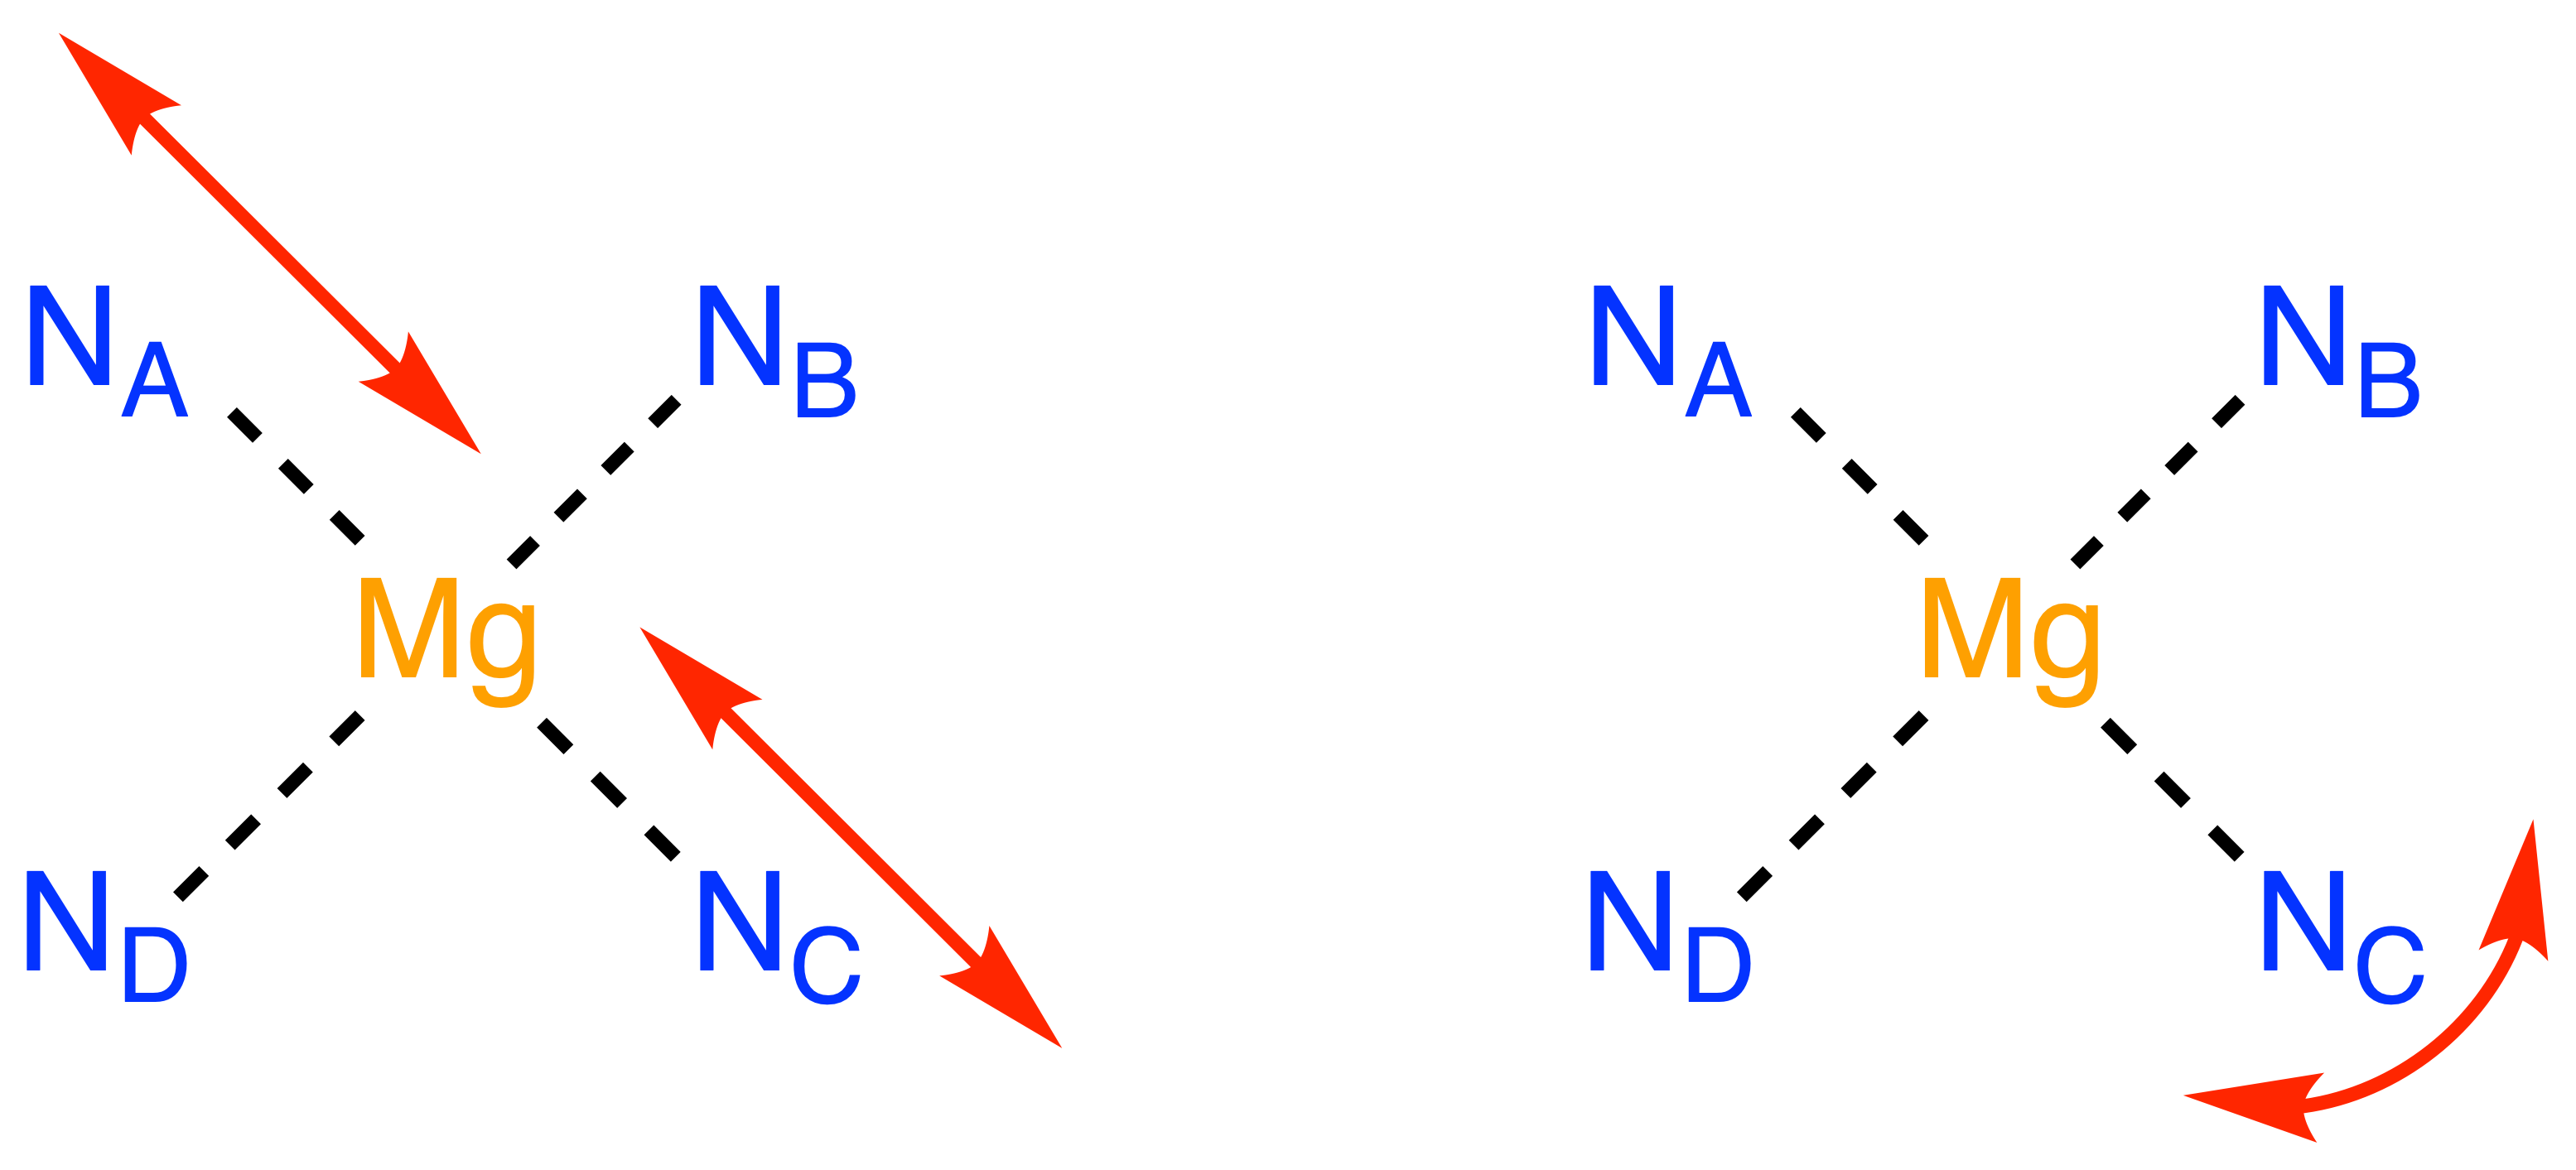
\includegraphics[scale=1.5]{chapters/4_chl_xtb/D4h_symmetry.png}
    \caption{Normal modes of the nitrogen-magnesium centre of chlorophyll that have
    $D_{4h}$-$D_{2h}$ (left) and $D_{4h}$-$C_{s}$ (right) symmetry breaking components.}
    \label{fig:D4_sym_breaking}
\end{figure}

\begin{figure}
    \centering
    \includegraphics[scale=0.55]{../../Year_2/BChla_Qy/qy_length_scan.png}
    \caption{Change in the $N_A$-$N_C$ displacements along the set of GFN1-xTB 
    normal modes for a chlorophyll molecule truncated at the phytyl tail.}
    \label{fig:qy_length_scan}
\end{figure}

\begin{figure}
    \centering
    \includegraphics[scale=0.55]{../../Year_2/BChla_Qy/qy_angle_scan.png}
    \caption{Change in the $N_A$-$Mg$-$N_C$ angle along the set of GFN1-xTB normal
    modes for a chlorophyll molecule truncated at the phytyl tail. The smaller variance
    than in figure \ref{fig:qy_length_scan} led this metric to not be used in normal
    mode choices.}
    \label{fig:qy_angle_scan}
\end{figure}

Normal modes that would also have this symmetry breaking component were identified
by how much the $N_A$-$N_C$ displacement would change along each normal mode. A plot of these
values, as well as the moving average, is shown in figure \ref{fig:qy_length_scan}.
A similar scan was made of the $N_A$-$Mg$-$N_C$ angle, however less variance in
this value was found and the peak positions did not match previously reported frequencies
for strong coupling. Normal modes with the largest $N_A$-$N_C$ were then chosen 
for the transition properties scan. The normal modes that were chosen had frequencies 
at 669.6, 701.7, 733.3, 745.5, 755.1, 1105.0, 1107.0, 1122.2, 1142.9, 1320.3, 1361.8 
$\text{cm}^{-1}$, which roughly correspond to previously identified normal modes
with frequencies of around 728 and 1156 $\text{cm}^{-1}$ \cite{Kim2020}.

The geometry was propagated for each selected normal mode such that the sum of
all atomic displacements from the optimised geometry was in units of 1 \AA{}.
This was done up to 3 \AA{} as it was found for most normal modes the energy 
difference between the optimised geometry and 3 \AA{} displaced geometry was greater
than the thermal energy at 300 K. Alternatively, in an environment at 300 K, a chlorophyll 
system would not be expected to deform past these boundaries. At each increment,
the \Qy transtion energy and dipole were calculated using chl-xTB, as well as TD-DFT
with PBE0/Def2-SVP and CAM-B3LYP/Def2-SVP levels of theory, \dscf and eigenvalue 
differences (both using PBE0/Def2-SVP). A quadratic fit was made for each of the
response methods and is shown in figures \ref{fig:mode_83} to \ref{fig:mode_135}. 
Some points for the \dscf method are not shown due to issues with excited state 
convergence.

\begin{figure}
    \centering
    \includegraphics[scale=0.5]{../../Year_2/BChla_Qy/mode_83.png}
    \caption{Transition energies and dipole magnitudes for the \Qy transition for
    geometries of truncated chlorophyll along the 83rd normal mode (frequency 669.6
    $\text{cm}^{-1}$).}
    \label{fig:mode_83}
\end{figure}

\begin{figure}
    \centering
    \includegraphics[scale=0.5]{../../Year_2/BChla_Qy/mode_85.png}
    \caption{Transition energies and dipole magnitudes for the \Qy transition for
    geometries of truncated chlorophyll along the 85th normal mode (frequency 701.7
    $\text{cm}^{-1}$).}
    \label{fig:mode_85}
\end{figure}

\begin{figure}
    \centering
    \includegraphics[scale=0.5]{../../Year_2/BChla_Qy/mode_88.png}
    \caption{Transition energies and dipole magnitudes for the \Qy transition for
    geometries of truncated chlorophyll along the 88th normal mode (frequency 733.3
    $\text{cm}^{-1}$).}
    \label{fig:mode_88}
\end{figure}

\begin{figure}
    \centering
    \includegraphics[scale=0.5]{../../Year_2/BChla_Qy/mode_90.png}
    \caption{Transition energies and dipole magnitudes for the \Qy transition for
    geometries of truncated chlorophyll along the 90th normal mode (frequency 745.5
    $\text{cm}^{-1}$).}
    \label{fig:mode_90}
\end{figure}

\begin{figure}
    \centering
    \includegraphics[scale=0.5]{../../Year_2/BChla_Qy/mode_91.png}
    \caption{Transition energies and dipole magnitudes for the \Qy transition for
    geometries of truncated chlorophyll along the 91st normal mode (frequency 755.1
    $\text{cm}^{-1}$).}
    \label{fig:mode_91}
\end{figure}

\begin{figure}
    \centering
    \includegraphics[scale=0.5]{../../Year_2/BChla_Qy/mode_129.png}
    \caption{Transition energies and dipole magnitudes for the \Qy transition for
    geometries of truncated chlorophyll along the 129th normal mode (frequency 1105.0
    $\text{cm}^{-1}$).}
    \label{fig:mode_129}
\end{figure}

\begin{figure}
    \centering
    \includegraphics[scale=0.5]{../../Year_2/BChla_Qy/mode_130.png}
    \caption{Transition energies and dipole magnitudes for the \Qy transition for
    geometries of truncated chlorophyll along the 130th normal mode (frequency 1107.0
    $\text{cm}^{-1}$).}
    \label{fig:mode_130}
\end{figure}

\begin{figure}
    \centering
    \includegraphics[scale=0.5]{../../Year_2/BChla_Qy/mode_132.png}
    \caption{Transition energies and dipole magnitudes for the \Qy transition for
    geometries of truncated chlorophyll along the 132nd normal mode (frequency 1122.2
    $\text{cm}^{-1}$).}
    \label{fig:mode_132}
\end{figure}

\begin{figure}
    \centering
    \includegraphics[scale=0.5]{../../Year_2/BChla_Qy/mode_135.png}
    \caption{Transition energies and dipole magnitudes for the \Qy transition for
    geometries of truncated chlorophyll along the 135th normal mode (frequency 1142.9
    $\text{cm}^{-1}$).}
    \label{fig:mode_135}
\end{figure}

It can be seen that chl-xTB predicts PBE0 transition energies with a high degree
of accuracy. Transition dipole magnitudes are predicted with worse accuracy, but
still capture the general behavior of PBE0 results well. chl-xTB consistently 
predicts PBE0 energies to within the same level of accuracy as achieved in the 
parameterisation test set. From the quadratic fits it can be seen that the gradients, 
turning points and curvature are well aligned between PBE0 and chl-xTB, especially
compared to \dscf and eigenvalue difference. It is also clear how important the
transition density scaling factor is in achieving accuracy for the transition dipole
magnitudes, with \dscf and eigenvalue difference being well above the region where
PBE0 and CAM-B3LYP values sit.

\afterpartskip
\subsection{Predicting Absorption Spectra}
\label{subsec:absorption_spectra}

So far all of the benchmark tests on chl-xTB have been for gas phase systems and
have no environmental effects. However in reality chlorophyll molecules would be
embedded in many different environments, for example the LH2 protein. Although the
training set took structures that have been perturbed by the LH2 protein, it is 
important to test the behavior of properties predicted by chl-xTB when explicitly
embedded. The obvious case for this would be predicting an absorption spectra for
chlorophyll when embedded by an explicit solvent. Additionally, it should be tested
whether the method could work for chlorophyll systems other than BChla. This would
be important for future investigations into chlorophyll systems, but for the remaining
work here it is not as important, and so is not investigated fully.

The absorption spectra was calculated using frames from an MD trajectory of chlorophyll
\emph{a} in an explicit diethyl ether solvent. An explicit solvent was used to account
for inhomogeneous broadening in the spectrum. The MD was performed with the
\code{OpenMM} toolkit. Force-field parameters for the chlorophyll were taken from
a bespoke parameterisation for photosystem II \cite{Zhang2012}, with the rest of
the system using the OpenForceField. The structure for chlorophyll was taken from
the same source as the bespoke force-field, and packed with explicit solvent using
the tools in the \code{Mistral} package. Equilibration and production steps were 
done with a Langevin integrator set to 300 K  and a time-step of 0.5 femtoseconds.
The system energy was minimized before running a 10 ps equilibration. Frames were
then taken from a 2 ns simulation time, with structures taken every picosecond.

Transition properties were calculated for chlorophyll structures from every frame.
This was done with the chl-xTB method, as well as PBE0 and CAM-B3LYP TD-DFT, both
using the Def2-SVP basis set. Experimental data for the absorption spectra were 
also taken from Katz \emph{et. al} \cite{Strain1963}. Embedding effects were
included in the chl-xTB Fock matrix with a particle mesh Ewald method. The real 
space term was calculated using \code{QCORE}, whereas the more complicated reciprocal
space spline term was calculated with the \code{HelPME} library. The absorption 
spectra for each method are shown as the absorption probability at excitation energies
in nanometers, normalized such that the areas under all spectra matched that of 
the experimental spectrum. The absorption spectra, both with and without a single-parameter
shift of excitation energies, can be seen in figure \ref{fig:chl_diethyl_ether}.

\begin{figure}
    \centering
    \includegraphics[scale=0.55]{../../Year_2/AbsorptionSpectra/cla_diethyl_ether_spectra.png}
    \caption{Predicted and experimental absorption spectrum of chlorophyll in diethyl 
    ether, only in the $Q$ band region. Predicted spectra are shown without energy
    shifts on the left, and with an energy shift to match the experimental absorption
    maximum on the right. All spectra are normalized to have equal areas.}
    \label{fig:chl_diethyl_ether}
\end{figure}

chl-xTB performs equally well as TD-DFT methods at simulating absorption spectra,
although constrained by the limits of the method and the training data. It can be
seen that the chl-xTB line-shape is similar in position and width to the PBE0 method.
This is highly encouraging, as the functional groups on chlorophyll A can have a
large effect on the \Qy transition, and so the good agreement here provides evidence
that important chemical features are captured in systems outside the training set.
Despite being trained purely on BChl a geometries (from \emph{Rsp. Acidophilus}),
it is able to predict the spectrum of solvated Chl \emph{a} (from \emph{Thermostichus vulcanus})
to within the same level of expected error (compared to PBE0). Although the chl-xTB
line-shape is wider than the experimental spectrum, the CAM-B3LYP and PBE0 lines
are also wider and so chl-xTB is still within a reasonable expectation of accuracy.

All of the predicted spectra lack of the lower intensity peaks that are present 
in the experimental spectrum, resultant from other $Q$ transitions. The lack of $Q_x$ 
peaks are expected, due to these transitions not being included in the predicted 
spectra, however the lack of the other \Qy peak can be seen in all methods bar CAM-B3LYP.
There gives two explanations of why chl-xTB is missing this peak. First is that the
PBE0 data does not include this feature, and so it would be unreasonable to expect
it to be learnt from the training data. Second is that the training data include 
geometries from the LH2 complex, and so would not cover the conformations that give
this lower intensity peak in a diethyl-ether system. Including Bchla geometries
from different environments might fix this issue, but as this work only considers
light harvesting systems this is outside the current scope.

\section{Conclusions}
\label{sec:chl_conclusions}

It has been shown that novel approximations to the full linear-response eigenvalue
equation can give accurate predictions of transition properties from high-level 
methods, which when combined with efficient electronic structure methods can give
a very powerful tool for predicting transition properties. However it is clear that
limitations in the optimisation procedure create systemic issues with the final
method such as a lack of accuracy outside LH2 conformations.

For alternative studies, it may not have been necessary to include both the altered 
xTB framework and the novel response approximations. If alternative studies require
a lower the efficiency (i.e. fewer calculations), a low level DFT calculation may 
have been good enough to achieve the required accuracy. This approach may have also
been easier to parameterize, requiring less global parameters and more closely following
the sTDA formalism. However as stated in the introduction, the efficiency of the 
desired methods does require semi-empirical efficiency, and so studying the response
approximations outside of an xTB framework is not in the scope of this work.

Additionally the accuracy of the chl-xTB method against training data is most likely
in large part due to the specificity. In general this is not an issue as many complex
systems require highly specific treatment, especially for large scale systems such
as chlorophyll. Applying the optimisation workflow to another system may be expected
to work well on two conditions. First is how well a single transition character
could approximate higher order transitions. This is easily sketched out by comparing
other single transition methods, such as the \dscf and eigenvalue difference methods,
against any training data. Second is be how well the electronic structure can be 
improved by altering the H{\"u}ckel and scaling parameters. Altering parameters
in other GFN-xTB terms might be required for more complex systems, which would require
more training data to optimise.

Although any system other than of chlorophyll is outside the scope of this work, 
it would be beneficial to know how far the optimisation workflow can be pushed. 
With only a relatively small size of the training data required, reoptimization 
of the current parameters could be equally short as found with the approach here. 
Additionally, depending on the system, the training data could be improved by either
using a higher level method or by including a larger conformational range. By understanding
the limits of the protocol in greater detail, it would be known beforehand whether 
a candidate system and transition could be expected to work. Many studies that require
large numbers of calculations could be bootstraped in a similar fashion.

In terms of modelling light harvesting complexes, Chl-xTB fulfills all the required
criteria set out in the introduction. It is efficient enough to calculate a huge
volume of properties in a reasonable amount of time. Additionally the benefit of
using the xTB framework is that the memory and CPU requirements are fairly low.
This allows for good scaling on high performance computers, using chl-xTB in a 
highly parallelized program (discussed in more detail in chapter \ref{chap:LH2}).
Additionally the accuracy of the method overcomes the statistical crutches that
are used in other methods, making the models of light harvesting complexes far more
detailed and chemically meaningful.

Overall, chl-xTB performs as well as can be expected from choices made in collecting
the training data. Predictions of transition energies and transition dipoles are
reliably close to the PBE0 values, and well within the error between different high 
level DFT functionals. It could be expected that improvements in the training data 
would yield better accuracy. This might be done by extending the training data in 
either the conformational space, or by investigating other systems. Applying chl-xTB 
to light harvest models forms the subject of the next chapters.

